% \documentclass[CEJM,DVI]{cej} % use DVI command to enable LaTeX driver
\documentclass[CEJM,PDF]{cej} % use PDF command to enable PDFLaTeX driver
\usepackage{layout}
\usepackage{booktabs}
\usepackage{latexsym}
\renewcommand*\rmdefault{ppl}
\graphicspath{ {images/} }


\title{Predicting The Best Starting Price for Ebay Auctions}

\articletype{Course Project Milestone 1: Data Preparation and Future Plan} % Research Article, Review Article, Communication, Erratum




\author{Jiacheng~Liao\inst{1},
        Yi~Wan\inst{1},
        Shuang~Zhou\inst{1},
        Zhaoyin~Zhu\inst{2}
       }

%\shortauthor{F. Author, S. Author}

\institute{\inst{1}
           Department of Computer Science, New York University, New York, NY 10012, USA
           \inst{2}
           Division of Biostatistics, NYU School of Medicine, New York, NY 10016, USA
          }

\abstract{Online auctions are one of the most popular methods to buy and sell items on the internet. With more than 100 million active users globally, eBay is the world’s largest online marketplace, where anyone can buy and sell anything. In order to successfully selling products on ebay, a reasonable starting price does not only determine whether the product will be sold or not but also affects the profit you can make from the transaction. In this project, we use the historical auction data collected from eBay from April 2013 to the first week of May 2013 which contains information about 296,048 successful and unsuccessful auctions. Different statistical models and machine learning algorithms will be utilized to study online auction patterns and predict the starting price that maximizes profits. Furthermore, we will compare the performance of different methods and summarize the pros and cons in different situations.
}

\keywords{Ebay Auction \*\ Predictive Analytics \*\ Data Mining}

%\msc{XXXXX, YYYYY}

\begin{document}
\maketitle
%\baselinestretch{2}
\section{Introduction (Data and Business Understanding) }

EBay is the world’s largest marketplace for sports autographs, the vast majority of the site’s membership uses it to buy and/or sell items via auction format. The ability to provide a method to estimate auction sale prices is desirable to this community. Members of most communities related to collectibles have reported they most often try to predict how much an auction would sell for by performing a search for item and manually calculating the average sales price. In this project, our first objective is to determine whether an auction listing will result in a sale. In addtion, we aim to predict the final sales price as well as the best starting price using data mining techniques.


\section{Data Preparation}

Data Preparation is an crucial and time-consuming part of our data mining project. It involves selecting data to include, cleaning data to improve data quality, constructing new data that may be required, integrating multiple data sets, and formatting data. We first preprocessed the downloaded data sets using shell scripts. To gain more experience on feature selection, we have performed the selection procedure on all three tools used in the class, RapidMiner, Weka and R. With different algorithms and parameters, we get slightly different but generally consistent results. 

\subsection*{Data Preprocessing}
Before any data can be used for later feature reduction and selection, we preprocessed our data sets. Here the tool we use is shell scripts. Initially, the raw data consists of training sets and test sets. Since we intend to do cross-validation on the whole data set, we merge all the separate data sets as one complete sets. Then we carefully go through all the data attributes and deleted all that obviously contain meaningless or irrelevant information to our analysis, such as ebayID, sellerName, etc. In addition, some attributes with ambiguous meanings are also discarded. 


\subsection{Feature Selection Using Weka}
First, we perform feature selection in Weka. To enable Weka to better handle the data, the first step is establishing a nominal class label. Below is a snapshot of the method we use here to discretize the class field here, which is originally a numeric type with value 0 and 1.

{\centering
    \vspace{3 mm}
    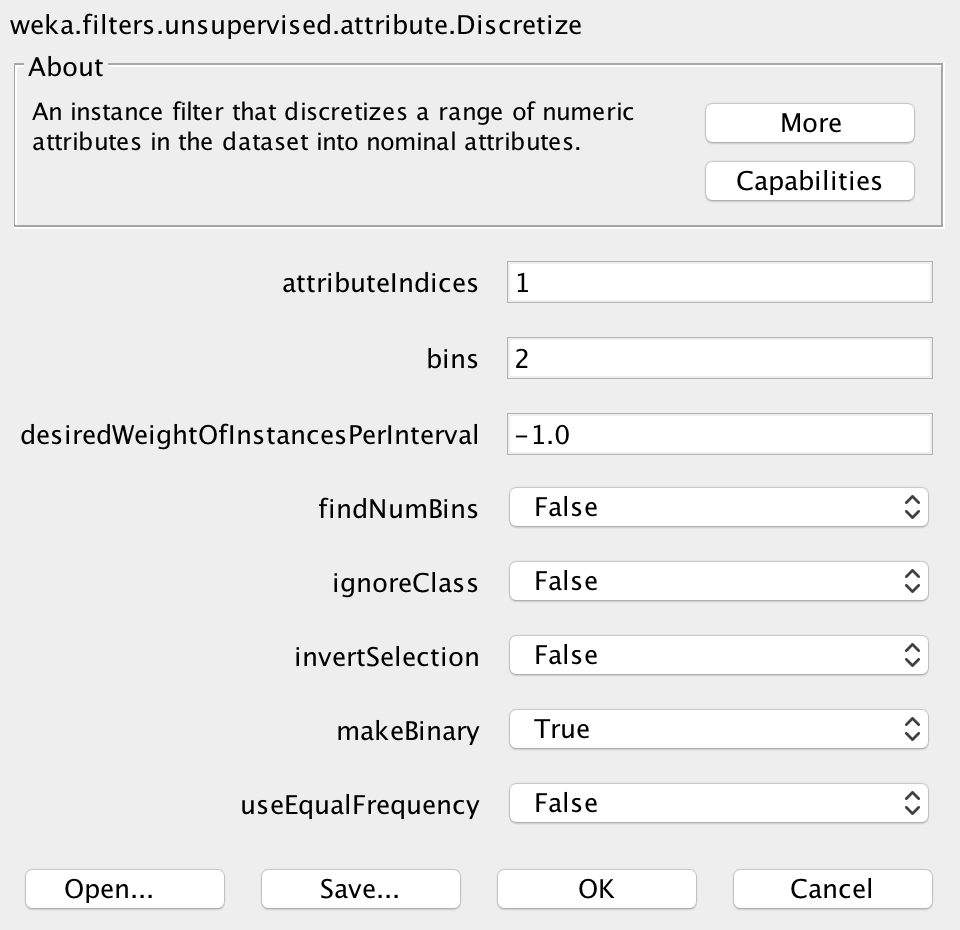
\includegraphics[scale=0.4]{weka-discretize_label_column.png}
    \par
}


Two algorithms are used in Weka: Information Gain and Feature Subset Selection. We first used Information Gain Algortihm and the result is as below. According to the information gain results we have, if we set the entropy threshold to 0.95, we will need the top 8 features.

{\centering
    \vspace{3 mm}
    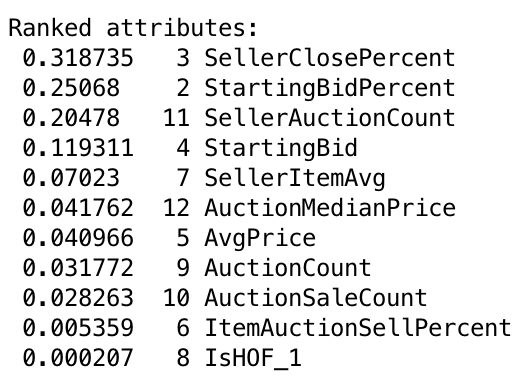
\includegraphics[scale=0.6]{weka-InfoGain.png}
    \par
}

Using the number of features obtained above, we set the number of features to 8 and try feature subset selection. We start with empty subset, and we use CfsSubsetEval as the evaluation of each subset, and we use GreedyStepWise search method, which basically select the best next feature based on current subset. Here is the result we get.

{\centering
    \vspace{3 mm}
    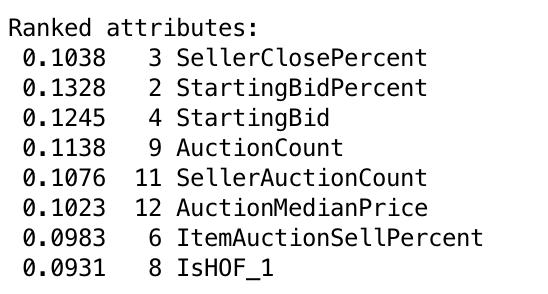
\includegraphics[scale=0.6]{weka-FilteredSubsetWithGreedyStepwise.png}
    \par
}



\subsection{Feature Selection Using R}
The caret R package provides tools automatically report on the relevance and importance of attributes in your data and even select the most important features for you. Here we perform three different feature selection method on our dataset. We use three kinds of filters to get a better sense of what attributes are more important, and we have the results below.\\

\textbf{Entropy based filter}
\begin{verbatim}
                    		 attr_importance 		 rank
StartingBidPercent         0.142113054                     5
SellerClosePercent         0.191431639                     2
StartingBid                0.071807352                     8
AvgPrice                   0.462173422                     1
ItemAuctionSellPercent     0.002012785                    10
SellerItemAvg              0.042062863                     9
IsHOF                      0.000000000                    11
AuctionCount               0.152471109                     4
AuctionSaleCount           0.098943728                     7
SellerAuctionCount         0.128577549                     6
AuctionMedianPrice         0.176666755                     3
\end{verbatim}
\mbox{}\\
\textbf{Chi-square based filter}
\begin{verbatim}
           attr_importance rank
StartingBidPercent          0.26196726                 5
SellerClosePercent          0.29670612                 2
StartingBid                 0.18784361                 8
AvgPrice                    0.47460475                 1
ItemAuctionSellPercent      0.06509426                10
SellerItemAvg               0.14541187                 9
IsHOF                       0.00000000                11
AuctionCount                0.26282938                 4
AuctionSaleCount            0.20983745                 7
SellerAuctionCount          0.24177050                 6
AuctionMedianPrice          0.29014051                 3
\end{verbatim}
\mbox{}\\
\textbf{Correlation based filter}
\begin{verbatim}
               attr_importance 	rank
StartingBidPercent          0.05002078                10
SellerClosePercent          0.62856687                 1
StartingBid                 0.16766258                 3
AvgPrice                    0.10793493                 6
ItemAuctionSellPercent      0.08816751                 7
SellerItemAvg               0.07423485                 8
IsHOF                       0.01689967                11
AuctionCount                0.11040403                 5
AuctionSaleCount            0.16330465                 4
SellerAuctionCount          0.07086579                 9
AuctionMedianPrice          0.18235711                 2
\end{verbatim}

As a result, we summarize all the three different methods and and compute average rank for each attribute. The result is presented in table \ref{r-rank}.


\begin{table}[h]
\centering
\caption{Feature Selection Using R Result}
\label{r-rank}
\begin{tabular}{@{}ccccc@{}}
\toprule
Attribute Name         & Entropy based filter & Chi-square based filter & Correlation based filter & Average Rank \\ \midrule
SellerClosePercent     & 2                    & 2                       & 1                        & 1.7     \\
AvgPrice               & 1                    & 1                       & 6                        & 2.7     \\
AuctionMedianPrice     & 3                    & 3                       & 2                        & 2.7     \\
AuctionCount           & 4                    & 4                       & 5                        & 4.3     \\
AuctionSaleCount       & 7                    & 7                       & 4                        & 6.0     \\
StartingBid            & 8                    & 8                       & 3                        & 6.3     \\
StartingBidPercent     & 5                    & 5                       & 10                       & 6.7     \\
SellerAuctionCount     & 6                    & 6                       & 9                        & 7.0     \\
SellerItemAvg          & 9                    & 9                       & 8                        & 8.7     \\
ItemAuctionSellPercent & 10                   & 10                      & 7                        & 9.0     \\
IsHOF                  & 11                   & 11                      & 11                       & 11.0    \\ \bottomrule
\end{tabular}
\end{table}


\subsection{Feature Selection Using RapidMiner}
First we choose a feature selection method from RapidMiner. Here we use Forward Selection. Forward selection operator selects the most relevant attributes of the given ExampleSet through a highly efficient implementation of the forward selection scheme. 

Forward selections uses wrapper method to select attributes. Basically, it starts with an empty attribute set. It them add one attribute to run the model and measures the performance. The process keep adding attributes to the model to see if there is performance gain. Depending on the parameter set, it will terminate until there is no performance improvement or no significant performance improvement. Here we also use cross-validation to measure the performance of the model as well as the current attributes set the operator. 

For predicting the whether the given item can be sold or not, we use several classification algorithms, including: Naive Bayes, Decision Tree, Random Forest, Rule Induction, Neural net, Logistic Regression, Support Vector Machine. We will consider efficiency and prediction accuracy for each model to decide which one to adopt. 

\subsubsection{Naive Bayes modeling}
{\centering
    A. The attribute weight
    \vspace{3 mm}
    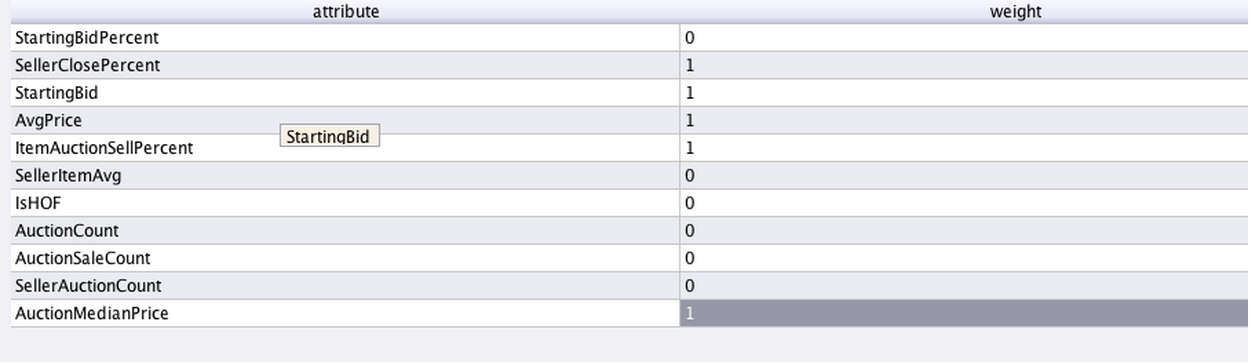
\includegraphics[scale=0.6]{rm-nb-aw.png}
    \par
}


{\centering
    B. The prediction model result and auc curve
    \vspace{3 mm}
    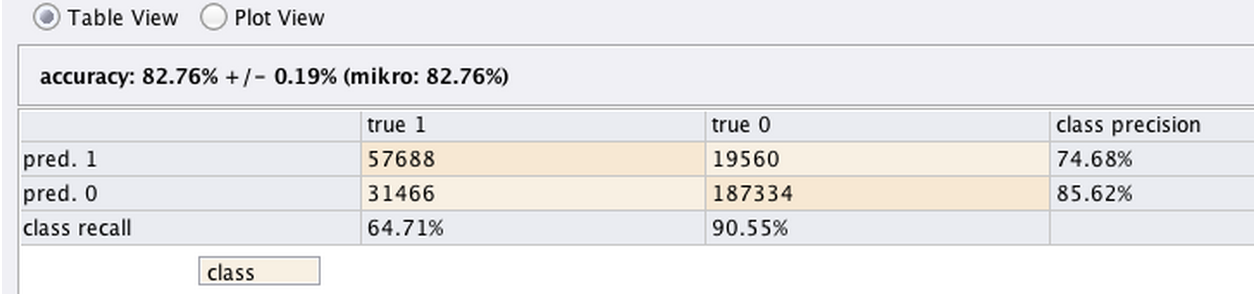
\includegraphics[scale=0.6]{rm-nb-perf.png}
    \vspace{3 mm}
    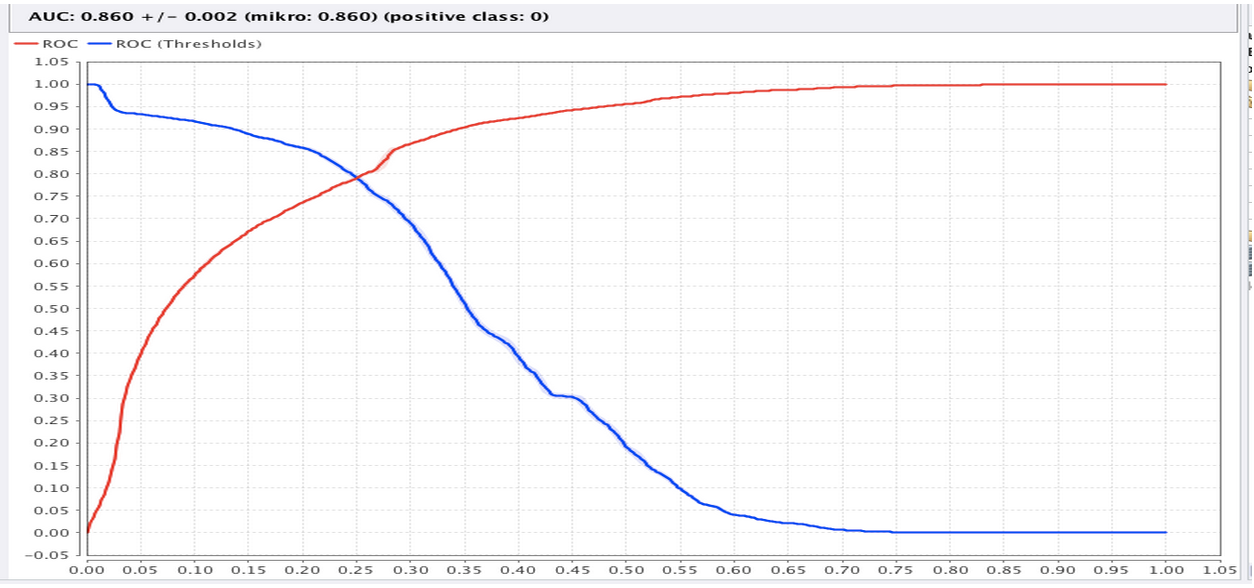
\includegraphics[scale=0.6]{rm-nb-auc.png}
    \par
}

\subsubsection{Decision Tree modeling}
{\centering
    A. The attribute weight
    \vspace{3 mm}
    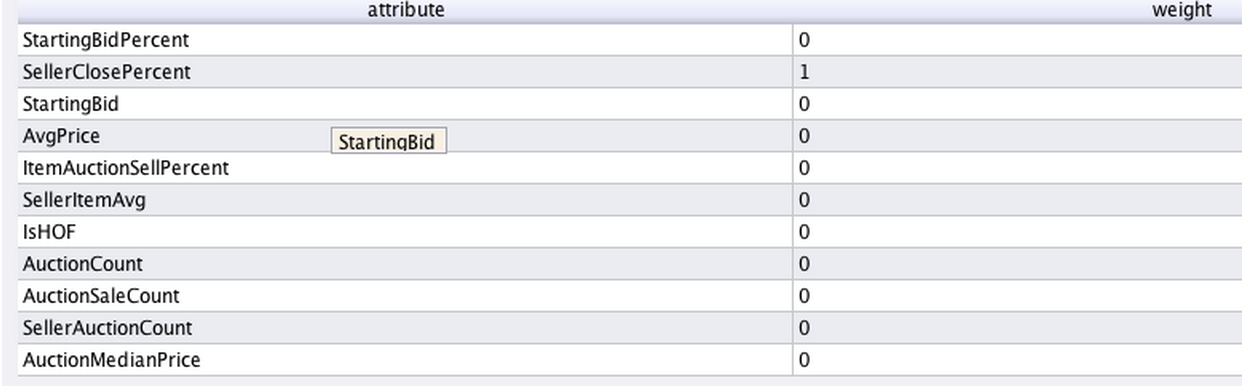
\includegraphics[scale=0.6]{rm-dec-aw.png}
    \par
}


{\centering
    B. The prediction model result and auc curve
    \vspace{3 mm}
    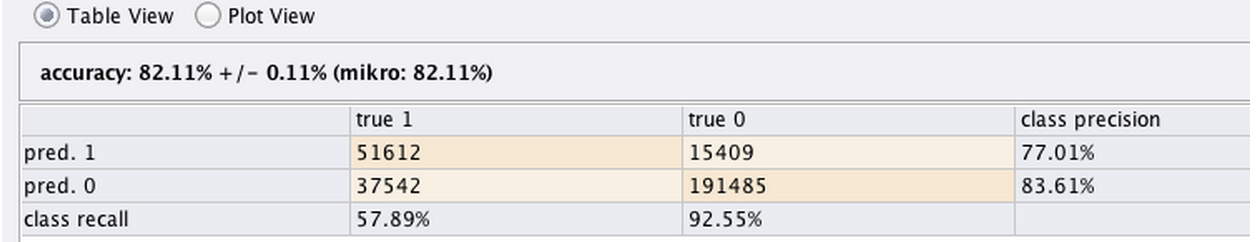
\includegraphics[scale=0.6]{rm-dec-perf.png}
    \vspace{3 mm}
    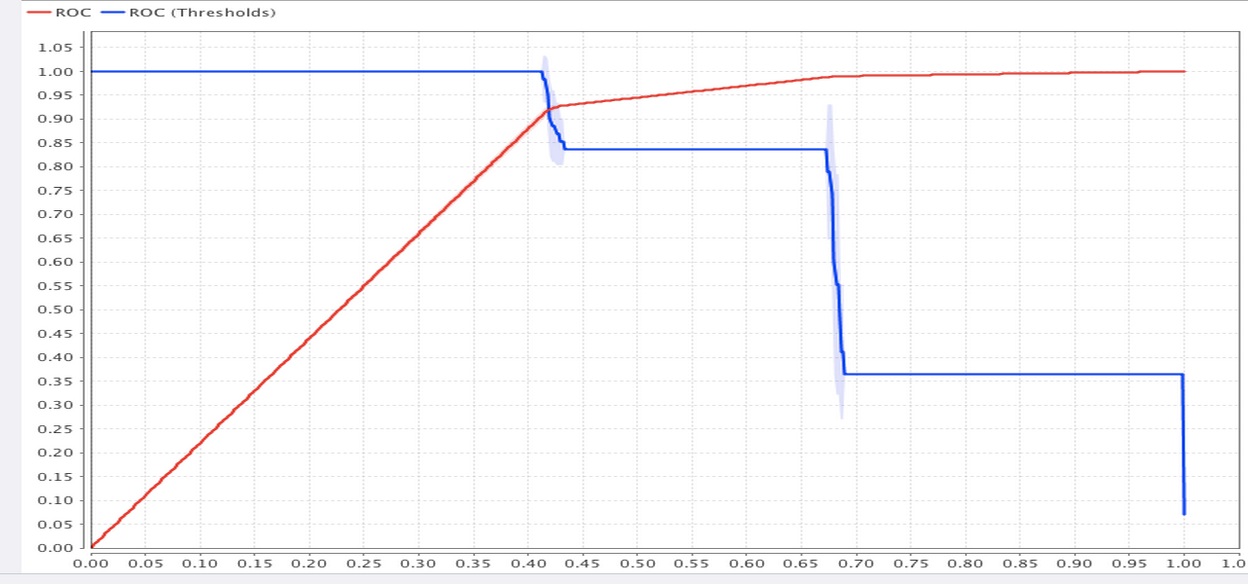
\includegraphics[scale=0.6]{rm-dec-auc.png}
    \par
}

\subsection{Other Methods}
The other methods including Random Forest, Rule Induction, Neural net, Logistic Regression, Support Vector Machine takes a very long time to finish (more than one hour). Since the dataset we are using is not very large, we consider them not suitable for our problem.


\section{Team Members Responsibilities and Plan for the Next Phase}

Right now, all group members are actively participate in the project. An approximate list of each team members' responsiblity is:
\begin{itemize}
\item Jiacheng Liao: data preprocessing, report write-up
\item Yi Wan: data preprocessing, feature selection in Rapidminer
\item Shuang Zhou: data preprocessing, feature selection in Weka
\item Zhaoyin Zhu: data preprocessing, feature selection in R
\end{itemize}

For the next phase,we intend to build different models to make predictions. We plan to apply various statistical machine learning model and use corss-validation to test each model. Also, we would study some economic aspects of the auction theory to help us build the model.



\section{Modeling (ToDo)}

Modeling involves selecting suitable modeling techniques, generating test designs to validate the model, building predictive models and assessing these models.


A predictive model is a mathematical function that predicts the value of some output variables based on the mapping between input variables. Historical data is used to train the model to arrive at the most suitable modeling technique. For example, a predictive model might predict the risk of developing a certain disease based on patient details. Some commonly used modeling techniques are as follows: Regression analysis that analyzes the relationship between the response or dependent variable and a set of independent or predictor variables. Decision trees that help explore possible outcomes for various options. Cluster analysis that groups objects into clusters to look for patterns. Association techniques that discover relationships between variables in large databases.

\section{Evaluation (ToDo)}
Evaluation involves evaluating the results against the business success criteria defined at the beginning of the project.


\section{Deployment (ToDo)}
Deployment involves consolidating the findings, determining what might be deployed and planning the monitoring and maintenance required to keep the model relevant.

\section{Conclusion (ToDo)}
TODO


\section*{Acknowledgements}

The author(s) would like to thank some institutions for support and so on.


\begin{thebibliography}{9}

\bibitem{data-mining}Han, Jiawei, Micheline Kamber, and Jian Pei.\textit{ Data mining: concepts and techniques: concepts and techniques}. Elsevier, 2011.

\bibitem{mining-mass} Rajaraman, Anand, and Jeffrey D. Ullman. \textit{Mining of massive datasets}. Vol. 77. Cambridge: Cambridge University Press, 2012.

\bibitem{pre-dummy} Bari, Anasse, Mohamed Chaouchi, and Tommy Jung. \textit{Predictive analytics for dummies}. John Wiley \& Sons, 2014.	

\bibitem{lecture} Bari, Anasse. Predictive Analytics Course Lecture Notes. 2015 Fall.

\bibitem{r-feature}  Brownlee, Jason. Feature Selection with the Caret R Package. http://machinelearningmastery.com/feature-selection-with-the-caret-r-package/

\bibitem{ebay-auction} Grossman, Jay. Predicting eBay Auction Sales with Machine Learning.

Retrived from http://jaygrossman.com/post/2013/06/10/Predicting-eBay-Auction-Sales-with-Machine-Learning.aspx


\end{thebibliography}

\end{document}
